% Chapter 2: Background

% Length: aim for 10-15 pages

This chapter presents the different background topics of the thesis work, which are the long-tailed datasets, model architectures \textit{Convolutional Neural Networks (CNN)} and \textit{Vision Transformers (VT)}, the deep long-tailed learning methods \textit{Class Re-balancing (CR)}, \textit{Information Augmentation (IA)}, 
and \textit{Module Improvement (MI)}. These topics will be explained for the reader.

\todo{Mention image classification, as it is the primary goal of this thesis.} 

% ===============================================================================
% LT Datasets

\section{Long-Tailed Datasets}
\label{sec:lt-datasets}
Long-tailed datasets pose significant challenges in deep learning, as they represent an extreme form of class imbalance. Addressing these challenges is central to this thesis, which explores methods to improve model performance on underrepresented classes. This section outlines the structure of long-tailed distributions and their implications.

A balanced dataset is one where all classes are evenly represented, whereas imbalanced datasets feature varying sample sizes across classes. Long-tailed datasets are characterized by a significant class imbalance, where a few dominant classes account for most samples (head classes), while the majority of classes are underrepresented (tail classes) as depicted in Figure \ref{fig:lt_distribution}. This  distribution is common for real-world datasets \cite{Newman_2005, liu2019largescalelongtailedrecognitionopen}. For example, the iNaturalist, a popular benchmark for image classification, exhibits a long-tailed distribution of species \cite{vanhorn2018inaturalistspeciesclassificationdetection}. Other benchmarks are constructed by sampling from datasets such as ImageNet \cite{ImageNet2009} by using a Pareto distribution, which simulates long-tailed class distributions with a power-law decay \cite{zhang2023deep, dealvis2024surveydeeplongtailclassification,cao2019learningimbalanceddatasetslabeldistributionaware}.

CIFAR100-LT \cite{cao2019learningimbalanceddatasetslabeldistributionaware}, derived from the CIFAR-100 dataset \cite{krizhevsky2009learning}, serves as the primary dataset for the experiments conducted in this thesis. CIFAR-100 is a widely used benchmark in classification research due to its diverse class representation and manageable size. It consists of 60,000 32x32 color images divided into 100 classes, each with 600 samples. These are further split into 500 training images and 100 testing images per class. CIFAR100-LT is created by reducing the number of samples in certain classes of CIFAR-100 following an exponential decay en sample sizes, given by:

\begin{equation}
    \label{eq:exp}
    n_i = n_{max}\cdot \text{IR}^{\frac{i-1}{C-1}}
\end{equation}

Where $n_i$ is the number of samples in class $i$, $n_{max}$ is the number of samples in the most frequent class, IR is the imbalance ratio, and $C$ is the total number of classes \cite{kaidic_ldam_drw}.

Other long-tailed datasets follow a Pareto distribution with number of samplers per class as followed \cite{liu2019largescalelongtailedrecognitionopen}:

\begin{equation}
    \label{eq:pareto}
    f(C) = \frac{\alpha C_{\text{m}}^\alpha}{C^{\alpha + 1}}, \quad C \geq C_{\text{m}}, \quad \alpha > 0
\end{equation}

Here, $\alpha$ is the shape parameter, $C_{\text{m}}$ is the scale parameter representing the minimum possible class index, and $C$ is the class index. A larger $\alpha$ results in a more severe imbalance.

\begin{figure}[ht]
    \centering
    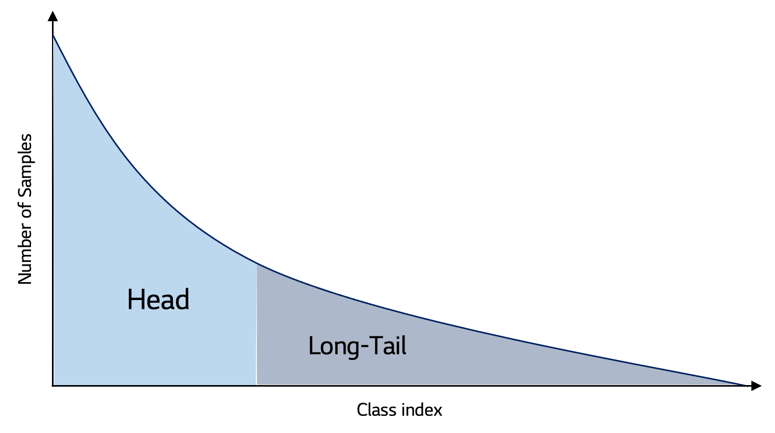
\includegraphics[width=0.8\textwidth]{Images/long_tail_distribution.png} 
    \caption{Illustration of a long-tailed distribution. Figure from \cite{lgresearch257}.}
    \label{fig:lt_distribution} % Use a unique label for referencing the figure
\end{figure}

Class imbalance has a profound impact on model performance compared to evenly distributed datasets \cite{vanhorn2017deviltailsfinegrainedclassification, cui2019classbalancedlossbasedeffective}. Deep networks trained on long-tailed datasets often exhibit biased performance, favoring head classes while performing poorly on tail classes \cite{zhang2023deep}. Zhang et al. (2023) provide a comprehensive survey of methods addressing this challenge, categorizing current approaches into three main groups: class re-balancing, information augmentation, and module improvement. These methods will be further explored in section \ref{sec:lt_methods}. 


% ===============================================================================
% Model architechtures

\section{Model Architecures}
\label{sec:model_arch}
Deep learning has revolutionized image classification by introducing models capable of learning complex patterns and representations from data. Among these, Convolutional Neural Networks (CNNs) and Vision Transformers (ViTs) are chosen as the primary architectures used in this thesis due to their performance on image classification tasks. This section provides a theoretical foundation for these models, focusing on the specific architectures utilized: MobileNetV2 \cite{sandler2018mobilenetv2}, ResNet50V2 \cite{he2016}, and ConvNeXt Base \cite{todi2023convnext} as the CNN architectures, and ViT-B/16 \cite{dosovitskiy2021imageworth16x16words} as the ViT architecture.

\todo{A brief summary of the relevance of the chosen architectures so that the reader knows why they are included.}

% ===============================================================================
% DNNs

\subsection{Introduction to Deep Neural Networks}
\label{sec:intro_DNN}
Before the introduction of Convolutional Neural Networks (CNNs) and, more recently, Vision Transformers (ViTs), the standard approach for image classification involved flattening a two-dimensional image matrix into a one-dimensional array and passing it through a Multilayer Perceptron (MLP), also known as a feed-forward neural network. MLPs are fully connected neural networks composed of an input layer, output layer, and one or more hidden layers. Being fully connected means that each neuron in a given layer is connected to all neurons in the next layer, forming a dense network. These connections are associated with weights and biases, which the network learns during training. Input features are fed into the input layer, propagated through hidden layers that add complexity to model nonlinear relationships, and yield predictions in the output layer. Known as universal approximators, MLPs can approximate any continuous function given sufficient neurons in the hidden layers \cite{zhang2023dive,HORNIK1989359}.

To illustrate the structure of a neural network, figure \ref{fig:dnn_layers} shows an example of a feed-forward neural network with three input neurons, two hidden layers, each with four neurons, and two output neurons. This architecture could be used, for instance, to classify images of cats and dogs based on three input features, such as height, weight, and width of the animals. The input propagates through the network, with each neuron computing a weighted sum of its inputs followed by an optional nonlinearity. The final output is a prediction, where the class corresponding to the neuron with the highest value is chosen.

\begin{figure}[ht]
    \centering
    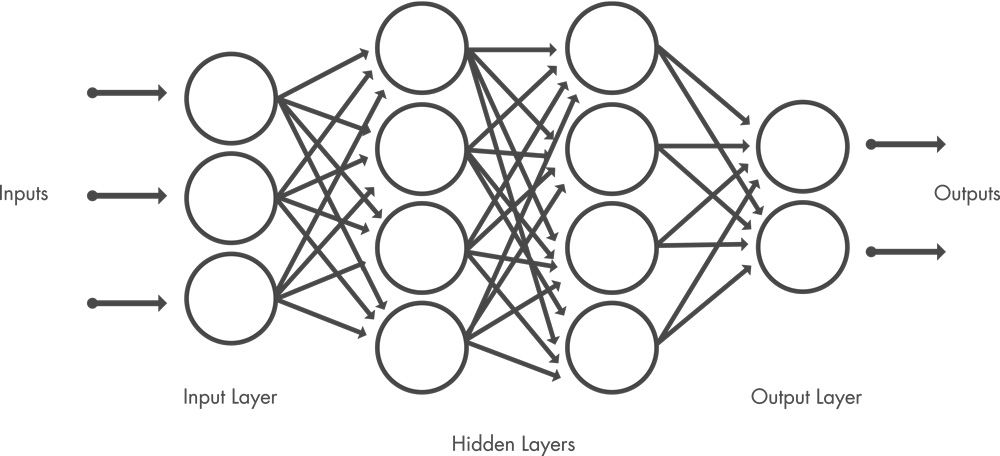
\includegraphics[width=0.8\textwidth]{Images/cnn_layers.jpg} 
    \caption{Layers of a neural network. Figure from \cite{mathworks_cnn}. \todo{Make this figure.}}
    \label{fig:dnn_layers}
\end{figure}

However, this simple neural network becomes insufficient for more complex problems, such as image classification, as it requires an increasing number of parameters. For instance, a $224\times 224$ RGB image flattened is very large, making MLPs parameter-heavy and inefficient. The limitations of MLPs were addressed by Convolutional Neural Networks (CNNs), which introduced convolutional and pooling layers to effectively preserve and utilize the spatial information of pixels in two-dimensional images \cite{zhang2023dive}.

\todo{Include how the weights are updated with gradients based on the loss function.}

% ===============================================================================
% CNNs

\subsection{Convolutional Neural Networks}
\label{sec:CNNs}
Convolutional Neural Networks (CNNs) \cite{lecun1995} were introduced to address the limitations of MLPs for image-related tasks. Unlike MLPs, which treat input features as independent, CNNs are designed to recognize patterns in images by applying local filters through convolutional layers, and thereby preserving the two dimensional input of an image, preserving the idea that nearby pixels are related \cite{lecun1998,NIPS2012_c399862d,zhang2023dive}. 

CNNs consist of several core components, as illustrated in Figure~\ref{fig:cnn_illustration}. 

\todo{write this section}
They have three main layers: convolutional layers, pooling layers, and a fully connected layer. The convolutional layer is the first layer, and serves to extract local features by applying filters to small regions of an image, while pooling layers reduce the spatial dimensions of feature maps, providing invariance to small translations. The CNN can be made up of multiple convolution and pooling layers, but the fully connected layer will be the final layer. Activation functions introduce nonlinearity, allowing the network to capture complex patterns. At the final stage, fully connected or global pooling layers aggregate the extracted features into predictions, enabling tasks such as classification or segmentation.

\todo{What is a convolution?}
\todo{Inductive bias}


\begin{figure}[ht]
    \centering
    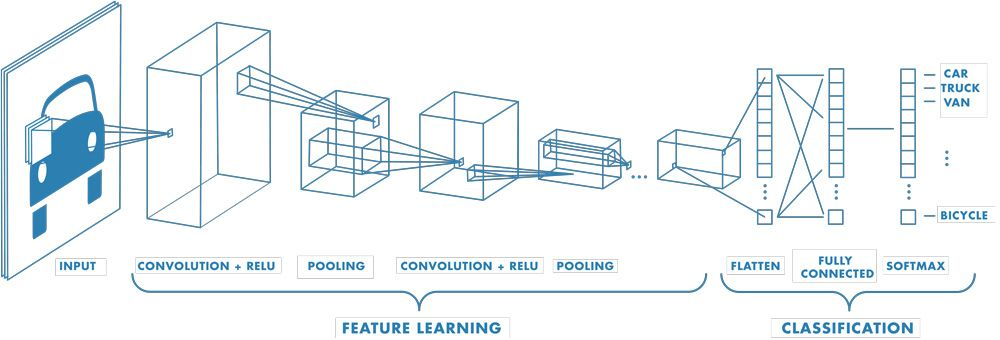
\includegraphics[width=0.8\textwidth]{Images/CNN_illustration.jpg} 
    \caption{Illustration of a convolutional neural network. Figure from \cite{mathworks_cnn}. \todo{Make this figure.}}
    \label{fig:cnn_illustration}
\end{figure}

\todo{Tie to the models used for experiments in this thesis.}
\url{https://www.ibm.com/topics/convolutional-neural-networks}

CNNs gained popularity after the introduction of LeNet-5 by LeCun et al. in 1998 \cite{lecun1998} that demonstrated the potential of CNNs by recognizing handwritten digits. Later, AlexNet \cite{NIPS2012_c399862d} achieved a breakthrough by winning the ImageNet Challenge in 2012, demonstrating the potential of CNNs to handle large-scale image recognition tasks by deepening the architechtures and utilizing multiple GPUs for training. Subsequently, the evolution of CNNs has progressed through architectures such as VGGNet \cite{simonyan2015deepconvolutionalnetworkslargescale}, GoogLeNet \cite{szegedy2014goingdeeperconvolutions}, and ResNet \cite{he2015deepresiduallearningimage}, which have set the stage for the advancements seen in modern CNNs.

% ===============================================================================
% ResNet50

\subsubsection{ResNet50 Architecture}
\label{sec:resnet}
ResNet50 is a variant of the Residual Network (ResNet) architecture, developed by Microsoft Research (He et al.) in 2015 \cite{he2015deepresiduallearningimage}. The ResNet architecture was designed to address the vanishing and exploding gradient problem in deep networks. When training a deep neural network, as the number of layers increases, the gradients of the loss function with respect to the weight can potentially vanish or explode during backpropagation \cite{he2015deepresiduallearningimage}. This can lead to slow convergence or unstable updates.

In traditional CNNs, stacked layers learn a direct mapping $\mathcal{H}(x)$ of the input $x$ to the output. The introduction of residual layers, however, allows for the layer to fit a residual mapping, as illustrated in figure \ref{fig:res_learning}, where the network learns the residual function $\mathcal{F}(x) = \mathcal{H}(x) - X$. Isolating $\mathcal{H}(x)$ yields $\mathcal{H}(x) = \mathcal{F}(x) + x$, meaning that the input $x$ is passed through a skip connection. This architecure reduces the complexity of the optimization process, as the network only has to model the residual component $\mathcal{F}(x)$ rather than the full mapping $\mathcal{H}(x)$ \cite{he2015deepresiduallearningimage}.

\begin{figure}[ht]
    \centering
    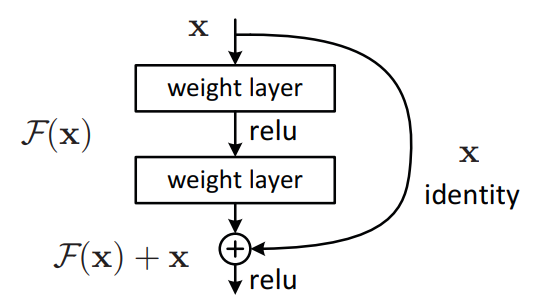
\includegraphics[width=0.5\textwidth]{Images/res_learn.png} 
    \caption{Residual Learning. Figure from \cite{he2015deepresiduallearningimage}. \todo{Make this figure.}}
    \label{fig:res_learning}
\end{figure}

The residual network is formed by stacking multiple layers of residual blocks, as the one depicted in figure \ref{fig:res_learning}. The ResNet architecture can have a varying number of layers, and, as the name implies, the ResNet50 variant has 50 layers. Other architecures include ResNet-34, ResNet-101, and ResNet-152 \cite{he2016identitymappingsdeepresidual}. 

The ResNet50 implementation consist of 1 convolutional layer, 4 stages of bottleneck residual blocks with layers [3, 4, 6, 3], global average pooling, and finally a fully connected layer for classification\cite{torchvision-resnet}, as seen in figure \ref{fig:resnet50}. 

\begin{figure}[ht]
    \centering
    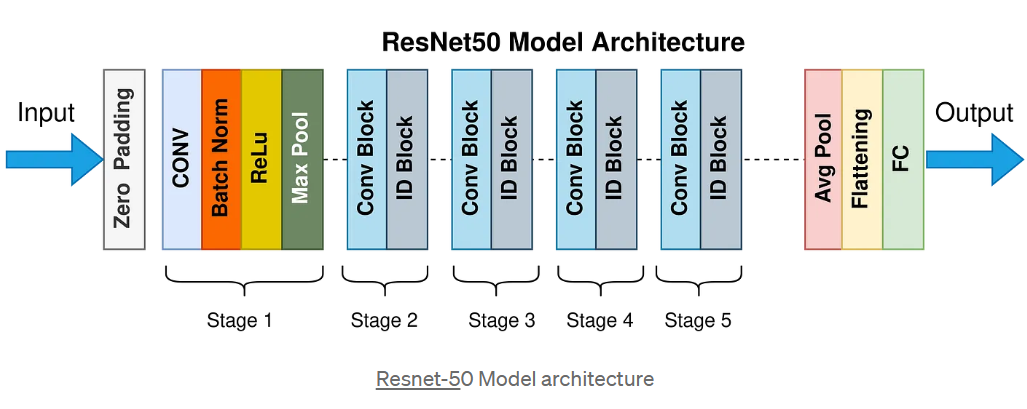
\includegraphics[width=0.9\textwidth]{Images/resnet50.png} 
    \caption{ResNet50 Architecture. Figure from \url{https://towardsdatascience.com/the-annotated-resnet-50-a6c536034758}. \todo{Make this figure.}}
    \label{fig:resnet50}
\end{figure}

% ===============================================================================
% MobileNetV2

\subsubsection{MobileNetV2 Architecture}
\label{sec:mobilenet}
MobileNetV2 introduced by Sandler et al. \cite{sandler2018mobilenetv2} is a lightweight CNN model designed primarily to balance model accuracy and computational efficiency, making it suitable for mobile or embedded devices. Building upon the original concepts of MobileNetV1 \cite{howard2017mobilenetsefficientconvolutionalneural}, MobileNetV2 preserves the use of depthwise separable convolutions, a method for reducing the parameters and floating-point operations, while introducing a novel element known as the inverted residual structure. 

% \begin{figure}[ht]
%     \centering
%     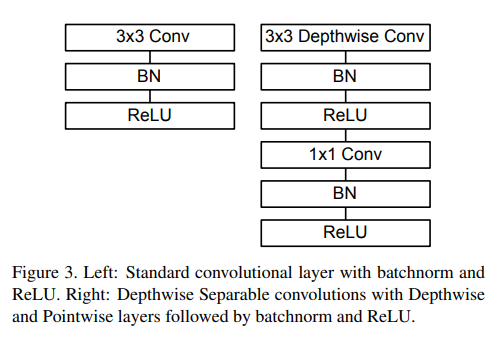
\includegraphics[width=0.8\textwidth]{Images/mobilenet_structure.png} 
%     \caption{Illustration of the MobileNetV1 structure. Figure from \cite{howard2017mobilenetsefficientconvolutionalneural}. \todo{Make this figure.}}
%     \label{fig:MobileNetV1_structure}
% \end{figure}

\paragraph{Inverted Residual Blocks}
While traditional residual connections described above allow for identity mapping and improved gradient flow, MobileNetV2 employs an inverted residual structure \cite{sandler2018mobilenetv2}. Instead of mapping from a high-dimensional representation down to a lower-dimensional bottleneck, then reconstructing features at the output, inverted residual blocks begin with a low-dimensional input and expand it to a higher-dimensional space before applying a depthwise convolution. After spatial filtering, the representation is projected back down to a low-dimensional space. This approach, illustrated in Figure \ref{fig:residual}, helps preserve crucial information and maintain a rich feature space without substantially increasing computational cost. The use of a linear bottleneck (i.e., no nonlinear activation in the low-dimensional projection) also helps prevent the destruction of useful information, further improving efficiency and accuracy.  

\begin{figure}[ht]
    \centering
    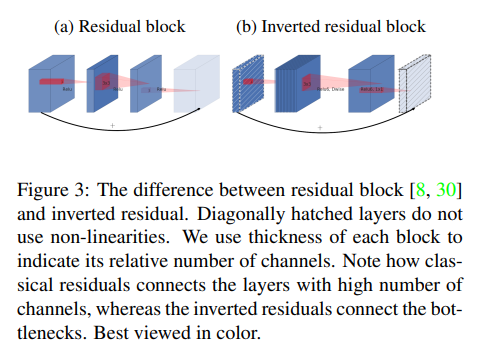
\includegraphics[width=0.8\textwidth]{Images/inverted_residual.png} 
    \caption{Residual and Inverted Residual Blocks. Figure from \cite{sandler2018mobilenetv2}. \todo{Make this figure.}}
    \label{fig:residual}
\end{figure}

\paragraph{Depthwise Separable Convolution}
Following MobileNetV1, MobileNetV2 relies on depthwise separable convolutions to factorize the convolution operation into two simpler operations \cite{howard2017mobilenetsefficientconvolutionalneural}: depthwise convolution and pointwise convolution as shown in figure \ref{fig:depthwise_sep_conv}. The depthwise convolution applies a single filter to each input channel, and the pointwise convolution (a $1\times 1$ convolution) then recombines the channels to produce the desired output. In comparison, a standard convolution both filtes and combines inputs into a new set of outputs. This approach reduces the parameter count and computational load, making the model suitable for devices with limited resources \cite{howard2017mobilenetsefficientconvolutionalneural,sandler2018mobilenetv2}.

\begin{figure}[ht]
    \centering
    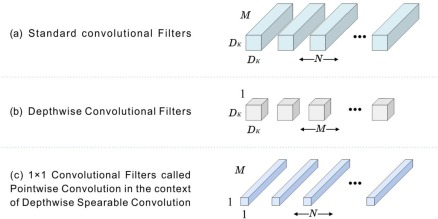
\includegraphics[width=0.8\textwidth]{Images/depthwise_separable_conv.jpg} 
    \caption{Depthwise Separable Convolution. Figure from \url{https://www.sciencedirect.com/topics/computer-science/depthwise-separable-convolution}. \todo{Make this figure.}}
    \label{fig:depthwise_sep_conv}
\end{figure}


\paragraph{Relevance}
\todo{Move to Methodology?}
In this thesis, MobileNetV2 represents an example of a modern, efficient CNN architecture. Its lightweight design makes it particularly attractive for applications where computational resources are limited. By including MobileNetV2 among the evaluated architectures, the performance is compared across varying complexity levels, providing insights into how efficiency-oriented designs fare against more complex models. This comparison is especially relevant if the application domain involves real-time processing or deployment on mobile or embedded devices.


% ===============================================================================
% Vision Transformers

\subsection{Vision Transformers}
\label{sec:ViTs}
\todo{Explain their advantages over CNNs for certain tasks.
Mention why they are relevant for handling long-tailed datasets.}

Transformers were introduced by Vaswani et al. in 2017 \cite{vaswani2023attentionneed}, and revolutionized the deep learning field, surpassing Recurrent Neural Networks (RNNs) for Natural Language Processing (NLP) tasks  \cite{v7labs-vit,vaswani2023attentionneed}. The design behind transformers is based on self-attention mechanism, allowing the model to weigh the significance of each part of input. As their design lack recurrence or convolutions, transformers use positional embeddings to represent the order of tokens in a sequence \cite{vaswani2023attentionneed}. Later, the Vision Transformer (ViT), an adaptation of the transformer architecture for image processing, was introduced by Dosovitskiy et al. (2021) \cite{dosovitskiy2021imageworth16x16words}. Here, images are represented as sequences including the class label as a learnable token for classification. The input image is divided into a sequence of patches, which are then flattened and liniarly embedded into a vector. The spacial information is preserved by adding positional encodings to the embeddings. Next, the sequence is fed into a transformer encoder identical to that introduced by Vaswani et al., consisting of alternating layers of Multi-head self-attention (MSP) and Multi-Layer Perceptron (MLP) blocks with Layer Norm (LN) applied before every block, and residual connection after every block. The final MLP layer acts as the classification head \cite{dosovitskiy2021imageworth16x16words}. The illustration in figure \ref{fig:vit_arch} shows the architecture of Vision Transformers.

\begin{figure}[h!]
    \centering
    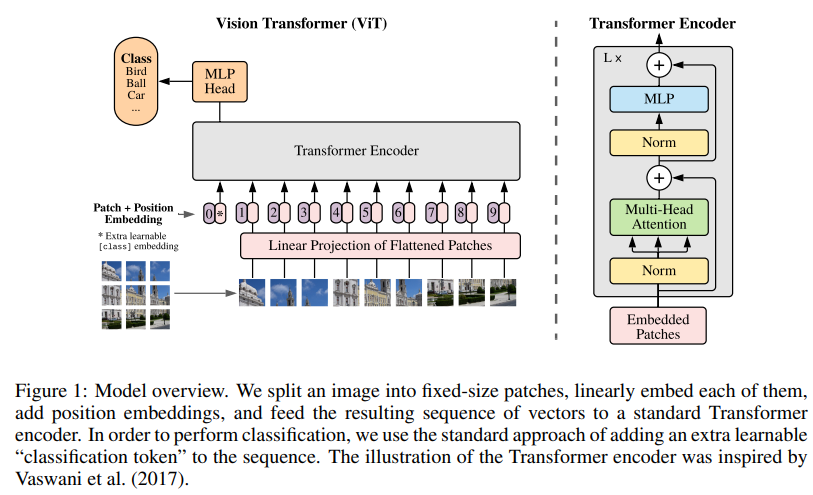
\includegraphics[width=0.8\textwidth]{Images/vit.png} 
    \caption{Vision Transformer architecture. Figure from \cite{dosovitskiy2021imageworth16x16words}. \todo{Make this figure.}}
    \label{fig:vit_arch}
\end{figure}

Unlike CNNs, ViTs have much less image-specific inductive bias \cite{dosovitskiy2021imageworth16x16words}. While the inductive bias in CNNs help the model generalize to unseen data \cite{kim2020inductivebias}, the ViT architecture does not include built-in assumptions about the structure of the data, only the MLP layers are local an translationally equivalent \cite{dosovitskiy2021imageworth16x16words}. As a result, ViTs require more training data to learn spacial relations compared with CNNs.

\todo{What made the ViT get SOTA? Why were they better than CNNs? \url{https://www.youtube.com/watch?v=QqejV0LNDHA}.}

% ===============================================================================
% ViT-B/16

\subsubsection{ViT-B/16 Architecture}
\label{sec:vitb16}
the ViT-B/16 is a Vision Transformer that leverages the transformer architecture for image classification \cite{dosovitskiy2021imageworth16x16words}, pre-trained on \todo{ImageNet-1K or ImageNet-21K?}. One of the main characteristics of the ViT-B/16 is that the input image consist of a fixed $16 \times 16$ patch size. It has 12 stacked encoder layers, each computing self-attention with 12 heads \cite{dosovitskiy2021imageworth16x16words}. Additionally, each layer includes an MLP, and skip-connections are applied around self-attention and MLP blocks for better gradient flow. LN is applied before the attention and MLP blocks. Afterwards, the appended class token is extracted, and a fully connected layer maps the token to the class prediction \cite{torchvision2024vitb16}. 


% ===============================================================================
% ConvNeXt Base

\subsubsection{ConvNeXt Base Architecture}
\label{sec:convnext}
ConvNext evolutionized the traditional CNN architecture by incorporating elements from ViTs, and was introduced by Liu et al. in 2022 \cite{liu2022convnet2020s}. 


ConvNeXt Base is a modernized CNN architecture inspired by insights from transformer-based models, designed to achieve competitive performance while retaining the efficiency of CNNs \cite{todi2023convnext}. Notable features include:

Simplified Design: Incorporates architectural refinements such as depthwise convolutions and LayerNorm.
Enhanced Efficiency: Balances accuracy and computational cost, bridging the gap between traditional CNNs and transformer-based models. 

Improvement from predecessors: integrating insights from ViTs.

\begin{figure}[ht]
    \centering
    \includegraphics[width=0.8\textwidth]{example-image} 
    \caption{Placeholder Image \todo{Make this figure.}}
    \label{fig:placeholder2}
\end{figure}

"The "Roaring 20s" of visual recognition began with the introduction of Vision Transformers (ViTs), which quickly superseded ConvNets as the state-of-the-art image classification model. A vanilla ViT, on the other hand, faces difficulties when applied to general computer vision tasks such as object detection and semantic segmentation. It is the hierarchical Transformers (e.g., Swin Transformers) that reintroduced several ConvNet priors, making Transformers practically viable as a generic vision backbone and demonstrating remarkable performance on a wide variety of vision tasks. However, the effectiveness of such hybrid approaches is still largely credited to the intrinsic superiority of Transformers, rather than the inherent inductive biases of convolutions. In this work, we reexamine the design spaces and test the limits of what a pure ConvNet can achieve. We gradually "modernize" a standard ResNet toward the design of a vision Transformer, and discover several key components that contribute to the performance difference along the way. The outcome of this exploration is a family of pure ConvNet models dubbed ConvNeXt. Constructed entirely from standard ConvNet modules, ConvNeXts compete favorably with Transformers in terms of accuracy and scalability, achieving 87.8 \% ImageNet top-1 accuracy and outperforming Swin Transformers on COCO detection and ADE20K segmentation, while maintaining the simplicity and efficiency of standard ConvNets." \url{https://paperswithcode.com/paper/a-convnet-for-the-2020s}


%====================================================================================
% Long-Tailed Methods

\section{Classic Long-Tailed Methods}
\label{sec:lt_methods}
\todo{Introduce the three methods (CR, IA, MI) with a brief explanation of their purpose.}

Following the paper \textit{Deep Long-Tailed Learning: A Survey} \cite{zhang2023deep}, the existing deep long-tailed learning methods are grouped into three main categories based on their technical approach: class re-balancing, information augmentation, and module improvement. These categories are further divided onto sub-categories: re-sampling, class-sensitive learning, logit adjustment, transfer learning, data augmentation, representation learning, classifier desing, decoupled training, and ensemble learning as shown on figure \ref{fig:lt_main_categories}. This thesis does not aim to examine all long-tailed methods, but aims to find a deep learning approach to a specific problem. The backgrounds of the methods used in this thesis are described in this section.

\todo{consider if it makes sense to mention all the methods in the survey paper, or just mention the class re-balancing.}

\begin{figure}[ht]
    \centering
    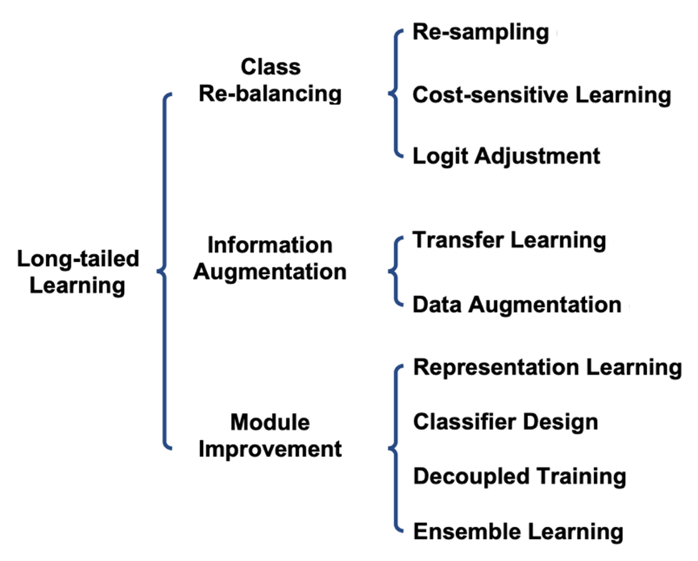
\includegraphics[width=0.8\textwidth]{Images/lt_methods_categories.png} 
    \caption{Long-tailed categories as described by \textit{Zhang et al.} \cite{zhang2023deep}.}
    \label{fig:lt_main_categories} % Use a unique label for referencing the figure
\end{figure}

\subsection{Class Re-balancing}
\label{sec:class_rebal}
The class re-balancing method aims to re-balance the effect of the imbalanced training dataset, and has three main sub-categories: re-sampling, class-sensitive learning, and logit adjustment \cite{zhang2023deep}. 

\todo{Include little about re-sampling, and focus on class-sensitive learning and an little on logit adjustment.}

\subsubsection{Re-sampling}
The traditional way to sample when training deep networks is using mini-batch gradient descent with random sampling. This means that each sample has an equal probability of being sampled. When sampling from an imbalanced dataset, samples from head classes naturally occur more often, and thus have higher chance of being sampled than samples from tail classes, making the resulting deep models biased towards head classes. Re-sampling is a method that adresses this problem by adjusting the number of samples per class in each sample batch for model training. 

\todo{Rewrite this section to closer resemble the related work.}

\subsubsection{Class-sensitive Learning}
Traditional training methods using the standard loss function, cross-entropy loss, can lead the model to be biased towards head classes, as the loss ignores class imbalance and thus generate an uneven amount of gradients for different classes \cite{zhang2023deep}. Consequently, tail classes are often misclassified. To address this imbalance, class-sensitive learning methods modify the loss function to pay more attention to minority classes, thus improving overall performance.

Two prominent categories of class-sensitive strategies are \emph{re-weighting} and \emph{re-margining}. Re-weighting involves adjusting the contribution of each class to the loss by multiplying them with different weights. By carefully selecting these weights, the model allocates a higher penalty to misclassification of underrepresented classes, thus re-balancing the training process \cite{zhang2023deep}. Re-margining, on the other hand, modifies the decision boundaries by introducing class-dependent margins, ensuring that minority classes have more room to establish discriminative features in the embedding space \cite{zhang2023deep, cao2019learningimbalanceddatasetslabeldistributionaware}.

In what follows, the theory behind several representative loss functions commonly used in class-sensitive learning is presented, beginning with an introduction to loss functions followed by the baseline Softmax Cross-Entropy loss. Subsequently, the theory behind multiple re-weighting schemes including Weighted Softmax Cross-Entropy, Focal Loss, Class-Balanced Loss, Balanced Softmax Loss, and Equalization Loss, as well as the re-margining method LDAM Loss. Each of these methods seeks to improve the imbalance in training through modifications that ultimately improve the classification performance on tail classes.

Table \ref{tab:loss_summary} summarizes the loss functions employed for class-sensitive learning used in this thesis, outlining their formulations and categorizations into re-weighting or re-margining strategies.


\begin{table}[H]
    \centering
    \caption{Summary of losses.}
    \label{tab:loss_summary}
    \begin{tabular}{|l|l|c|}
    \hline
    \textbf{Loss Name}       & \textbf{Formulation}                                                & \textbf{Type}        \\ \hline
    Softmax loss \cite{pytorch_crossentropy}             & $\mathcal{L}_{ce} = - \log(p_y)$                                              & -                   \\
    Focal loss \cite{lin2018focallossdenseobject}     & $\mathcal{L}_{fl} = -(1 - p_y)^\gamma \log(p_y)$                             & re-weighting        \\
    Weighted Softmax loss \cite{zhang2023deep}    & $\mathcal{L}_{wce} = - \frac{1}{\pi_y} \log(p_y)$                           & re-weighting        \\
    Class-balanced loss \cite{cui2019classbalancedlossbasedeffective} & $\mathcal{L}_{cb} = - \frac{1 - \gamma}{1 - \gamma^{n_y}} \log(p_y)$         & re-weighting        \\
    Balanced Softmax loss \cite{ren2020balancedmetasoftmaxlongtailedvisual} & $\mathcal{L}_{bs} = - \log\left( \frac{\pi_y \exp(z_y)}{\sum_j \pi_j \exp(z_j)} \right)$ & re-weighting        \\
    Equalization loss \cite{tan2020equalizationlosslongtailedobject} & $\mathcal{L}_{eq} = - \log\left( \frac{\exp(z_y)}{\sum_j \omega_j \exp(z_j)} \right)$    & re-weighting        \\
    LDAM loss \cite{cao2019learningimbalanceddatasetslabeldistributionaware}      & $\mathcal{L}_{ldam} = - \log\left( \frac{\exp(z_y - \Delta_y)}{\sum_j \exp(z_j - \Delta_j)} \right)$ & re-margining        \\
    \hline
    \end{tabular}
\end{table}


\paragraph{Introduction to Loss Functions}
Loss functions are a fundamental component in machine learning and deep learning \cite{zhang2023dive,Goodfellow-et-al-2016}. They serve as a measure of how far a model's predictions are from the actual values, where higher loss indicates greater prediction error, whereas a lower loss implies more accurate predictions. Thus, the goal of training a model is to minimize the loss. 

The loss function plays a crucial role, as it guides the model to adjust its parameters (weights and biases) through an optimization algorithm \cite{Goodfellow-et-al-2016}. The algorithm calculates the gradient of the loss function with respect to each parameter to determine how the parameter affect the loss. Afterwards, the model update its parameter to reduce the loss, following:

\begin{equation}
    \label{eq:gradient_update}
    w_{t+1} = w_t - \eta \frac{\partial L}{\partial w_t}
\end{equation}

Here, $w$ are the parameters, $\eta$ is the learning rate, and $L$ is the loss function. This is an iterative process, and continues until the loss reaches a minimum or the model converges.

From equation \eqref{eq:gradient_update}, the choice of loss function is critical as it influences the model's interpretation of prediction errors and parameter adjustment. For image classification tasks, the standard loss function is the cross-entropy loss combined with the softmax activation function \cite{zhang2023dive} described in the following.

\todo{This is the SGD. Include the Adam Optimizer.}

\paragraph{Softmax Cross-Entropy Loss}
The \emph{Softmax Cross-Entropy (CE) loss} is a fundamental building block in training deep classifiers and is widely regarded as the baseline in classification tasks \cite{zhang2023deep, cs231n, pytorch_crossentropy}. The softmax loss, as it is commonly known as, is the combination of the cross-entropy loss and the softmax activation function \cite{zhang2023dive,Goodfellow-et-al-2016}. First, the need of the softmax activation function will be decribed.

The \textit{Softmax} function transforms the raw output scores (logits) of the final layer of a neural network into a probability distribution over \( K \) classes. For an input \( \mathbf{z} = [z_1, z_2, \dots, z_K] \), the Softmax function for class \( i \) is defined as:

\begin{equation}
    P(y = i \mid \mathbf{z}) = \frac{\exp(z_i)}{\sum_{j=1}^{K} \exp(z_j)}
\end{equation}

Here, \( \exp(z_i) \) ensures that all values are positive, and dividing by the sum normalizes the probabilities so that they sum to 1. This normalization is crucial for classification, as it allows the network's outputs to represent the likelihood of each class.

The \textit{Cross-Entropy loss} measures the difference between the predicted probability distribution \( \mathbf{P} \) (produced by Softmax) and the true distribution \( \mathbf{y} \) (the one-hot encoded ground truth). It is defined as:

\begin{equation}
    \mathcal{L}_{\text{CE}} = -\sum_{i=1}^{K} y_i \log(P(y = i \mid \mathbf{z}))
\end{equation}

For a single example where the true class is \( c \), this simplifies to:

\begin{equation}
    \label{eq:ce_loss}
    \mathcal{L}_{\text{CE}} = -\log(p_y)
\end{equation}

This equation penalizes incorrect predictions by heavily weighting the log of the predicted probability for the true class. The loss is minimized when the predicted probability \( P(y = c \mid \mathbf{z}) \) approaches 1, indicating high confidence in the correct class.

While this approach provides a robust and stable training objective, it inherently treats all classes equally and does not account for class imbalance.


\paragraph{Weighted Softmax Cross-Entropy Loss}
The \emph{Weighted Softmax Cross-Entropy (WCE) loss} modifies the standard CE loss (equation \eqref{eq:ce_loss}) by introducing a weighting factor $w$. For multiclass classification, the CE loss it is multiplied by the inverse class frequencies $1/\pi_y$ \cite{zhang2023deep,lin2018focallossdenseobject}, given by:

\begin{equation}
    \label{eq:wce_loss}
    \mathcal{L}_{\text{WCE}} = -w \log(p_y) = - \frac{1}{\pi_y} \log(p_y)
\end{equation}

This weighted CE loss ensures that minority classes contribute more to the overall loss, addressing the imbalance during training.


\paragraph{Focal Loss}
\emph{Focal Loss} \cite{lin2018focallossdenseobject} addresses class imbalance by improving model performance on hard-to-classify examples by focusing on wrongly classified examples. The technique for this is called down-weighting, and uses the prediction probabilities to dynamically adjust the contribution of each sample to the loss. Well-classified examples with high probabilities $p_y$ are down-weighted by adding a modulating factor $(1 - p_y)^\gamma$ to the cross-entropy loss (eq. \eqref{eq:ce_loss}). Here, $\gamma \geq 0$ is a tunable focusing parameter. The Focal Loss modifies the CE loss by applying the inverse prediction probability as follows:

\begin{equation}
    \label{eq:focal_loss}
    L_{fl} = -(1 - p_y)^\gamma \log(p_y)
\end{equation}

This factor increases the weight of misclassified examples, ensuring the model prioritizes learning from challenging samples. Figure \ref{fig:focal_loss} shows how the focal loss for different values of $\gamma$. When $\gamma = 0$ the modulating factor equals 1, and the focal loss becomes the standard CE loss. The blue line in figure \ref{fig:focal_loss} represents the standard cross-entropy loss for $\gamma = 0$.

\begin{figure}[h!]
    \centering
    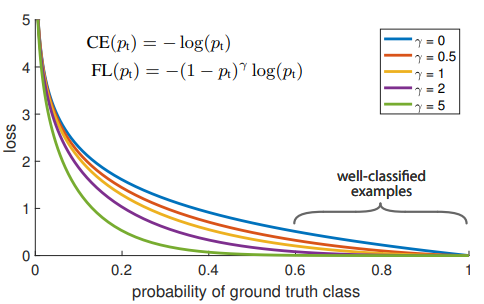
\includegraphics[width=0.6\textwidth]{Images/focal_loss.png}
    \caption{Figure from \cite{lin2018focallossdenseobject}. \todo{Make this figure}}
    \label{fig:focal_loss}
\end{figure}

\paragraph{Class-Balanced Loss}
\emph{Class-Balanced (CB) Loss} \cite{cui2019classbalancedlossbasedeffective} introduces a re-weighting strategy based on the effective number of samples per class to re-balance the loss.

Instead of simply using raw class frequencies, CB Loss estimates how much additional information new samples provide, acknowledging an information overlap among data, and as the number of samples increases, the marginal benefit of extracted features from new data diminishes. As illustrated in figure \ref{fig:cb_featue_space}, the feature space is the map of all possible data, and each sample occupies a part of the space. Collecting more samples of a class means that there is a probability that their features overlap, meaning that additional samples diminishes new information.
In feature space, the probability of newly sampled data with volume 1 is overlapping $p$, which means that the probability of adding new information to the feature space is $(1-p)$. 


\begin{figure}[h!]
    \centering
    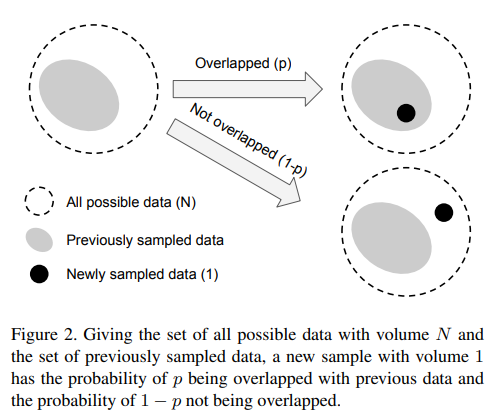
\includegraphics[width=0.6\textwidth]{Images/CB_feature_space.png}
    \caption{Figure from \cite{cui2019classbalancedlossbasedeffective}. \todo{Make this figure}}
    \label{fig:cb_featue_space}
\end{figure}

Cui et al. \cite{cui2019classbalancedlossbasedeffective} introduced the effective number of samples as the expected volume of samples, denoted $E_n$, where $n \in \mathbb{Z}_{>0}$ is the number of sampels. The effective number of samples 
is defined as:

\begin{equation}
    \label{eq:eff_num}
    E_n = \frac{1-\beta^n}{1-\beta}
\end{equation}

where $\beta = (N-1)/N$. The hyperparameter $\beta \in [0,1)$ determines how fast $E_n$ grows.

As a result, the CB loss introduces a class-balanced re-weighting term, inversely proportional to the effective number of classes. Adding the CB term to the standard softmax cross-entropy given in equation \eqref{eq:ce_loss} yield the following:

\begin{equation}
    \label{eq:cb_loss}
    L_{cb} = - \frac{1 - \beta}{1 - \beta^{n_y}} \log(p_y)
\end{equation}

where $n_y$ is the number of samples in the ground truth class $y$. Applying the inverse of the effective number ensures that minority classes contribute more to the total loss, as the effective number in equation \eqref{eq:eff_num} grows large for minority classes (small $n_y$) and small for majority classes (large $n_y$). When $\beta = 0$ the loss is equivalent to the CE loss. Contrary, when $\beta \longrightarrow 1$ the re-weighting effect grows.

\paragraph{Equalization Loss}
\emph{Equalization (EQ) Loss} \cite{tan2020equalizationlosslongtailedobject} aims to mitigate the over-suppression of tail classes, which occurs when these underrepresented classes serve predominantly as negative examples for the more frequent classes. The idea is to ignore the gradients for rare classes so that they are not excessively penalized when they appear as negatives, preventing their learned representations from being overshadowed. 

The EQ loss was designed for object recognition, but the authors decided to adopt the principles into image classification, officially called the \emph{Softmax Equalization (SEQ) Loss}, defined as: 

\begin{equation}
    \label{eq:EQ_loss}
    \mathcal{L}_{SEQL} = - \sum_{j=1}^{C} y_j \log(\tilde{p}_j)
\end{equation}

where

\begin{equation}
    \tilde{p}_j = \frac{e^{z_j}}{\sum_{k=1}^{C} \tilde{w}_k e^{z_k}}
\end{equation}

and the weight term is given by:

\begin{equation}
    \tilde{w}_k = (1 - \beta T_\lambda(f_k))(1 - y_k)
\end{equation}

Here, $y_j$ is the ground truth class, $z_j$ is the logit for class $j$, $f_k$ is the frequency of class $k$, \(T_\lambda(\cdot)\) is the threshold on class frequency, and \(\beta\) is a random variable taking value 1 with probability \(\gamma\) and 0 with probability \(1 - \gamma\).

\subsubsection{Logit Adjustment}
Logit adjustment is a class re-balancing technique that aims to optimize the class imbalance by adjusting the prediction logits \cite{menon2021longtaillearninglogitadjustment}, typically based on prior class probabilities. 
\todo{This is not finished}

\paragraph{Balanced Softmax Loss}
The \emph{Balanced Softmax (BS)} Loss modifies the standard softmax formulation by directly incorporating class priors $\pi_y$ into the logits before computing probabilities \cite{ren2020balancedmetasoftmaxlongtailedvisual}. Unlike approaches that operate solely in the loss space, BS Loss integrates class frequency adjustments at the probability computation stage, effectively neutralizing the bias introduced by imbalanced class distributions. The BS loss function is as follows:

\begin{equation}
    L_{bs} = - \log\left( \frac{\pi_y \exp(z_y)}{\sum_j \pi_j \exp(z_j)} \right)
\end{equation}

where $z_y$ represents the logit for the true class, $\pi_y$ is the class prior (e.g. normalized frequency of samples from class $y$), and the term in the denominator normalizes the probabilities across all classes while accounting for priors.

\todo{This is not finished}

\subsubsection{Re-margining}
Re-margining aims to solve class imbalance by improving classification by introducing margin between classes, encouraging higher margins between rare classes.

\todo{Describe margins in detail, and how they impact long-tailed learning.}

\paragraph{LDAM Loss}
The \emph{Label-Distribution-Aware Margin (LDAM)} Loss represents a class-sensitive approach based on re-margining rather than re-weighting \cite{cao2019learningimbalanceddatasetslabeldistributionaware}. 

Instead of altering the loss directly, LDAM modifies the margin applied to each class’ decision boundary, ensuring that minority classes have more “space” in the representation space to reduce misclassification.

\todo{This is not finished.}

"First, we propose a theoretically-principled label-distribution-aware margin (LDAM) loss motivated by minimizing a margin-based generalization bound. This loss replaces the standard cross-entropy objective during training and can be applied with prior strategies for training with class-imbalance such as re-weighting or re-sampling." 

\begin{equation}
    L_{ldam} = - \log\left( \frac{\exp(z_y - \Delta_y)}{\sum_j \exp(z_j - \Delta_j)} \right)
\end{equation}

From \cite{zhang2023deep}: To handle the class imbalance, re-margining
attempts to adjust losses by subtracting different margin factors for
different classes, so that they have a different minimal margin (i.e.,
distance) between features and the classifier. Directly using existing
soft margin losses [138], [139] is unfeasible, since they ignore the
issue of class imbalance. To address this, Label-Distribution-Aware
Margin (LDAM) [18] enforces class-dependent margin factors for
different classes based on their training label frequencies, which
encourages tail classes to have larger margins.

